\documentclass[a4paper,%
11pt,%
DIV12,
headsepline,%
headings=normal,
]{scrartcl}

\usepackage{bopc}
\usepackage{csvsimple}
\usepackage{todonotes}

%% ==================== ADAPT ACCORDINGLY ==================== %%

% args: first name, last name, matriculation number
\setAuthorOne{Pia}{Schwarzinger}{12017370}
\setAuthorTwo{Yahya}{Jabary}{11912007}

% set group size and group number, group size influences author formatting

% args: group size, group number (TUWEL)
\setGroup{2}{13}
%\setGroup{1}{X}

%% =========================================================== %%

\begin{document}

\maketitlepage

%% ================= SUBMISSION INFORMATION ================== %%

% Please fill out accordingly

%% ========================= REPORT ========================== %%

\setcounter{section}{1}
\section{The Tasks}

\setcounter{subsection}{1}
\begin{comment}
\textbf{}{Metrics}

\textit{Speedup}

\begin{itemize}
    \item What difference does parallelization make?
    \item $S_a(n,p) = \frac{T_{\text{seq}}(n)}{T_{\text{par}}(n,p)}$ = absolute speedup
    \item $S_r(n,p) = \frac{T_{\text{par}}(n, 1)}{T_{\text{par}}(n,p)}$ = relative speedup
\end{itemize}

Where:
\begin{itemize}
    \item $n$ = input size
    \item $p$ = number of processors
    \item $T_{\text{par}}(n,p)$ = parallel runtime
    \item $T_{\text{seq}}(n)$ = sequential runtime
\end{itemize}

\textit{Efficiency of Parallelization}

\begin{itemize}
    \item What difference does each processor make?
    \item $E(n,p) = \frac{T_{\text{seq}}(n)}{p \cdot T_{\text{par}}(n,p)} = \frac{1}{p} \cdot S_a(n,p)$
\end{itemize}
\end{comment}
\subsection{Compute Speed-up and Parallel Efficiency for 2 Instance Sizes }
Tables~\ref{tab:runtime_cs} and \ref{tab:runtime_cb} present the parallel runtime measurements and the respective speed-up and efficiency values for the cases $c_s$ and $c_b$.

\begin{table}[htb!]
 \centering 
\caption{\label{tab:runtime_cs}Runtime and speed-up of parallel Julia set generator for $c_s$ case.}
\begin{tabular}{rrrrr}
  \toprule
  size & p & mean runtime (s) & speed-up & par. eff.\\
  \midrule
  155 & 1 & 0.276419 & 1 & 1.42473 \\
  155 & 2 & 0.14614 & 1.89147 & 1.34742 \\
  155 & 4 & 0.0850049 & 3.2518 & 1.15824 \\
  155 & 8 & 0.0684728 & 4.03691 & 0.71894 \\
  155 & 16 & 0.0727858 & 3.7977 & 0.338169 \\
  155 & 24 & 0.0845242 & 3.27029 & 0.194137 \\
  155 & 32 & 0.0975262 & 2.8343 & 0.126191 \\
  \midrule
  1100 & 1 & 13.42 & 1 & 1.40137 \\
  1100 & 2 & 6.66189 & 2.01444 & 1.41149 \\
  1100 & 4 & 3.37751 & 3.97333 & 1.39203 \\
  1100 & 8 & 1.72664 & 7.7723 & 1.36149 \\
  1100 & 16 & 0.908652 & 14.7691 & 1.29356 \\
  1100 & 24 & 0.654567 & 20.5021 & 1.19713 \\
  1100 & 32 & 0.564249 & 23.7838 & 1.04156 \\
  \bottomrule
\end{tabular}
\end{table}

Keep in mind that while the speed-up was calculated using $p=1$ as the reference point, the parallel efficiency was calculated using an average of the sequential runtime, by running the following commands 3 times on the Hydra-cluster and averaging the results:

\begin{verbatim}
srun -p q_student -t 1 -N 1 -c 32 python3 julia.py --size 155 --nprocs 1 
# 155;20;1;0.39382300106808543
srun -p q_student -t 1 -N 1 -c 32 python3 julia.py --size 1100 --nprocs 1 
# 1100;20;1;18.806384983938187
\end{verbatim}

\begin{table}[htb!]
 \centering 
\caption{\label{tab:runtime_cb}Runtime and speed-up of parallel Julia set generator for $c_b$ case.}
\begin{tabular}{rrrrr}
  \toprule
  size & p & mean runtime (s) & speed-up & par. eff.\\
  \midrule
  155  & 1   & 0.394086         & 1        & 0.711286  \\
  155  & 2   & 0.210897         & 1.86862  & 0.66456   \\
  155  & 4   & 0.121818         & 3.23504  & 0.575259  \\
  155  & 8   & 0.0862224        & 4.57057  & 0.406373  \\
  155  & 16  & 0.0852527        & 4.62256  & 0.205497  \\
  155  & 24  & 0.0963721        & 4.08921  & 0.121191  \\
  155  & 32  & 0.108531         & 3.6311   & 0.0807109 \\
  1100 & 1   & 19.1049          & 1        & 0.68691   \\
  1100 & 2   & 9.67163          & 1.97536  & 0.678447  \\
  1100 & 4   & 4.90018          & 3.89883  & 0.669536  \\
  1100 & 8   & 2.4526           & 7.78967  & 0.66885   \\
  1100 & 16  & 1.28631          & 14.8525  & 0.637646  \\
  1100 & 24  & 0.900398         & 21.2183  & 0.607295  \\
  1100 & 32  & 0.746145         & 25.6049  & 0.549633  \\
  \bottomrule
\end{tabular}
\end{table}

Same as before, the parallel efficiency was calculated using an average of the sequential runtime, by running the following commands 3 times on the Hydra-cluster and averaging the results:

\begin{verbatim}
srun -p q_student -t 1 -N 1 -c 32 python3 julia.py --size 155 --nprocs 1 --benchmark 
# 155;20;1;0.2803074959665537
srun -p q_student -t 1 -N 1 -c 32 python3 julia.py --size 1100 --nprocs 1 --benchmark 
# 1100;20;1;13.123375411145389
\end{verbatim}

It's important to mention that we opted for logarithmic scaling on all y-axes in our graphs. This choice was made to enhance the visibility of function shapes/gradients over the marginal differences. However, it's crucial to be mindful that this results in each increment on the y-axis carrying significantly more weight.

Also: Going forward, we won't focus as much on how different seeds (S-Case vs. B-Case) change the Julia set fractal. This is because the load size has a much bigger impact on our results.  The results we've seen using different seeds have been very similar overall.

\subsubsection{Comparing: Absolute Speed-up vs. Number of Processes}

Figure~\ref{fig:nprocs-exectime} shows the absolute runtime in comparison to number of cores for both the S-case and B-case for two different sizes.

When comparing the impact of process count on runtime across datasets of differing sizes, we observe a few key trends.

With the larger dataset, there's a significantly sharper decline in runtime as we increase the number of processes/processors (these terms can \textit{approximately} be used interchangeably since setting \verb|chunksize=1| in Python's \verb|multiprocessing.Pool.map| means one task is mapped to each processor at a time - unless we have fewer cores than processes). Additionally, the runtime appears to flatten out as we increase the processor count. Conversely, with the smaller dataset, the decline in runtime is less pronounced, and starting from 8 processes, the overhead from fork syscalls actually outweighs the benefits of parallel computation, leading to an increase in runtime.

\subsubsection{Comparing: Relative Speed-up vs. Number of Processes}

Figure~\ref{fig:nprocs-speedup} demonstrates the relative speed up in comparison to number of cores for both the S-case and B-case for the same sizes as before.  

In our earlier analysis, we delved into the marginal decrease in runtime with the addition of each process. Essentially, this mirrors the concept of speedup, particularly when our baseline is at $p=1$. These findings reinforce what we've already discussed. However, it's important to note that the speedup gap between the two loads in the S-case is significantly larger. This likely stems from the increased number of iterations and computations needed per pixel to achieve convergence in the visualization.

\subsubsection{Comparing: Parallel Efficiency vs. Number of Processes}

The final figure~\ref{fig:nprocs-parefficiency} reveals a generally similar downward trend for both seed-cases in the significance per process with increasing number of processes (note that this is parallel efficiency, distinct from utilization). Additionally the decrease in parallel efficiency is a lot more pronounced in the smaller workload and comes very close to 0 as we reach $p=32$ in both seed-cases.
A crucial distinction lies in the initial baseline: in the B-case, the starting point for process efficiency is substantially lower (by a factor of 2) than the S-case. This significant difference in initial efficiency is not directly apparent from the graph itself and would require further examination of the data provided in the appendix. This could be another indicator for a higher compute-intensity in the S-case in addition to the gap previously observed in the speed-up.

\subsubsection{Discussion}

The findings highlight the importance of considering load size and parallel processing efficiency in computational analysis. Variation in seed choice has minimal impact compared to load size on results. Larger datasets show sharper decline in runtime with increasing processes, while smaller ones exhibit diminishing returns and eventual increase in runtime due to overhead. Parallel efficiency decreases with more processes, with the B-case starting at a lower efficiency than the S-case, indicating higher compute-intensity in the latter.

\begin{figure}[htb!]
    \centering
    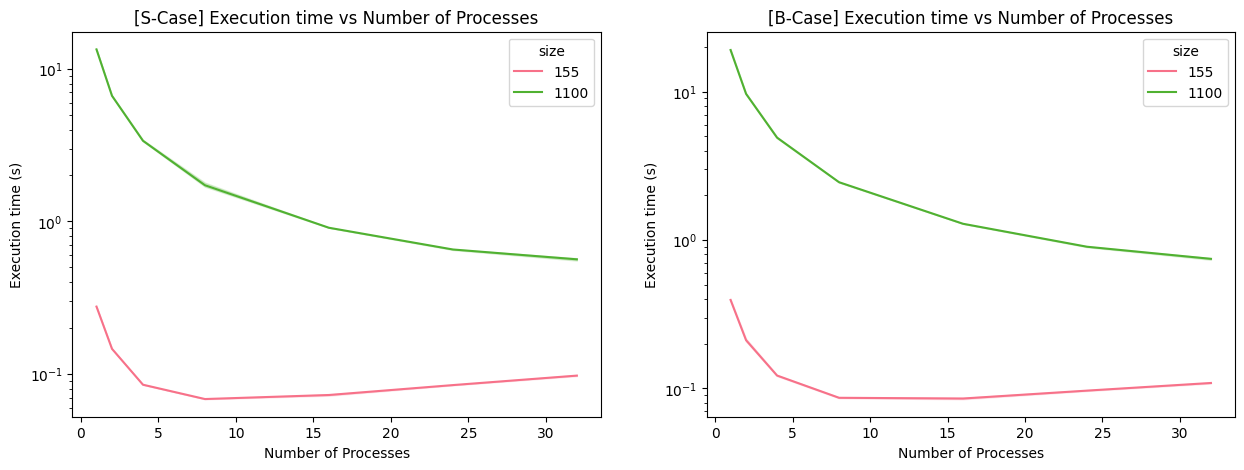
\includegraphics[width=\textwidth]{nprocs-exectime.png}
    \caption{Absolute Runtime vs. Number of Processes}
    \label{fig:nprocs-exectime}
\end{figure}

\begin{figure}[htb!]
    \centering
    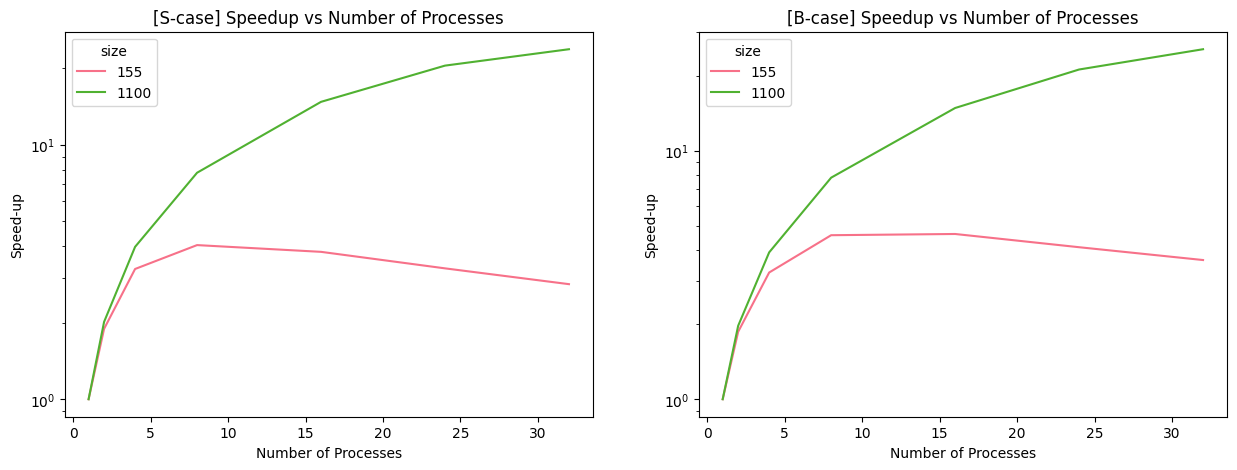
\includegraphics[width=\textwidth]{nprocs-speedup.png}
    \caption{Relative Speed-up vs. Number of Processes}
    \label{fig:nprocs-speedup}
\end{figure}

\begin{figure}[htb!]
    \centering
    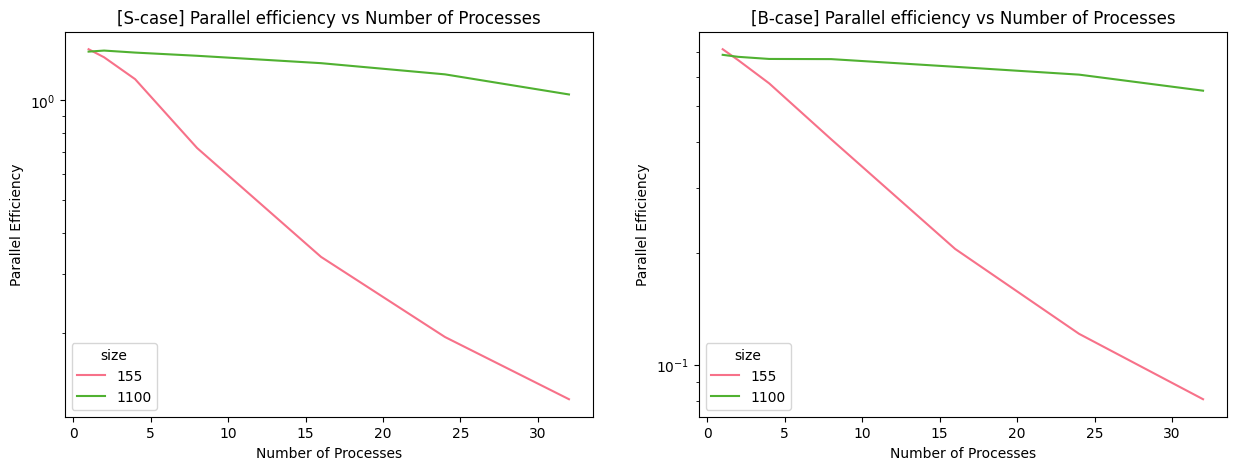
\includegraphics[width=\textwidth]{nprocs-parefficiency.png}
    \caption{Parallel Efficiency vs. Number of Processes}
    \label{fig:nprocs-parefficiency}
\end{figure}

\newpage
\clearpage
\subsection{Influence of Patch Size}

Table~\ref{tab:patch_size} presents the average runtimes in seconds of varying patch sizes, while keeping the number of cores and problem size the same. Again, the means are taken from three runs on the cluster. 

\begin{table}[h!]
\centering 
\caption{\label{tab:patch_size}Influence of patch size on mean runtime}
\begin{tabular}{rrrr}
\toprule
size & patch & nprocs & avg\_time \\
\midrule
950 & 1 & 32 & 59.680444 \\
950 & 5 & 32 & 2.439178 \\
950 & 10 & 32 & 0.827185 \\
950 & 20 & 32 & 0.589660 \\
950 & 55 & 32 & 0.649828 \\
950 & 150 & 32 & 1.791236 \\
950 & 400 & 32 & 5.347212 \\
\bottomrule
\end{tabular}
\end{table}

Figure~\ref{fig:patch_size} now visually shows the influence of the patch size on the mean runtime.

\begin{figure}[htb!]
    \centering
    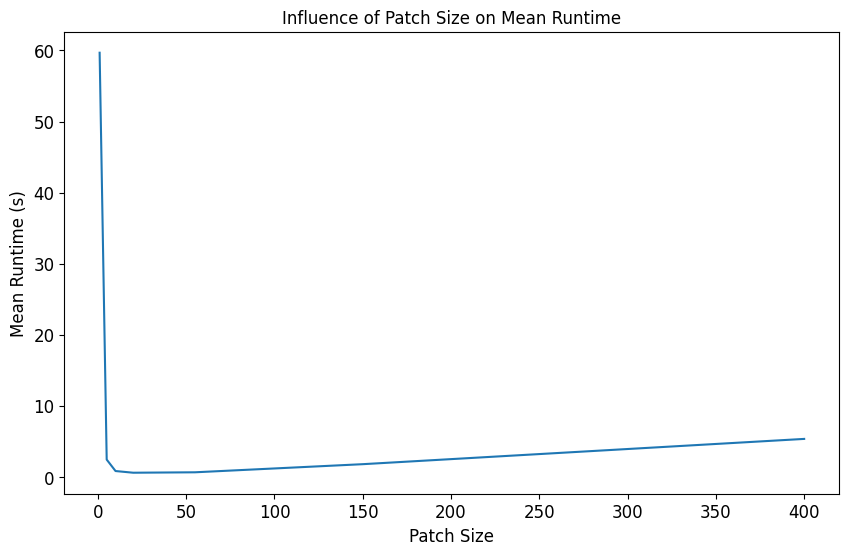
\includegraphics[width=0.7\textwidth]{template-2/patch_size_runtime.png}
    \caption{Mean Runtime vs. Patch Size - Influence of patch size}
    \label{fig:patch_size}
\end{figure}



As we can tell having a patch size of 1 leads to an extremely high runtime but drastically decreases once multiple patches are involved. This is because computational resources can be used more effectively and parallel processing can be improved. However, starting from 150 patches upwards, the runtime increases which is probably due to the overhead that comes with managing a large number of parallel processes.

\subsection{Finding the Best Patch Size}

In order to find the best possible patch size, table~\ref{tab:best_patch_size} and figure~\ref{fig:best_patch_size} present the results of our experiments. 

\begin{table}[htb!]
\centering 
\caption{\label{tab:best_patch_size}Best patch size}
\begin{tabular}{rrrr}
\toprule
size & patch & nprocs & avg\_time \\
\midrule
800 & 1 & 16 & 50.020686 \\
800 & 2 & 16 & 12.428263 \\
800 & 3 & 16 & 5.235198 \\
800 & 4 & 16 & 2.781848 \\
800 & 5 & 16 & 1.778088 \\
800 & 6 & 16 & 1.262205 \\
800 & 7 & 16 & 1.025805 \\
800 & 8 & 16 & 0.871605 \\
800 & 9 & 16 & 0.841269 \\
800 & 10 & 16 & 0.788733 \\
800 & 11 & 16 & 0.777117 \\
800 & 12 & 16 & 0.730836 \\
800 & 13 & 16 & 0.721792 \\
800 & 14 & 16 & 0.732972 \\
800 & 15 & 16 & 0.712528 \\
800 & 16 & 16 & 0.736369 \\
800 & 17 & 16 & 0.714250 \\
800 & 18 & 16 & 0.709131 \\
800 & 19 & 16 & 0.711833 \\
800 & 20 & 16 & 0.704302 \\
800 & 21 & 16 & 0.712072 \\
800 & 22 & 16 & 0.715015 \\
800 & 23 & 16 & 0.718865 \\
800 & 24 & 16 & 0.710345 \\
800 & 25 & 16 & 0.706855 \\
800 & 26 & 16 & 0.709854 \\
800 & 27 & 16 & 0.715558 \\
800 & 28 & 16 & 0.708274 \\
800 & 29 & 16 & 0.702031 \\
800 & 30 & 16 & 0.705310 \\
\bottomrule
\end{tabular}
\end{table}

\begin{figure}[h!]
    \centering
    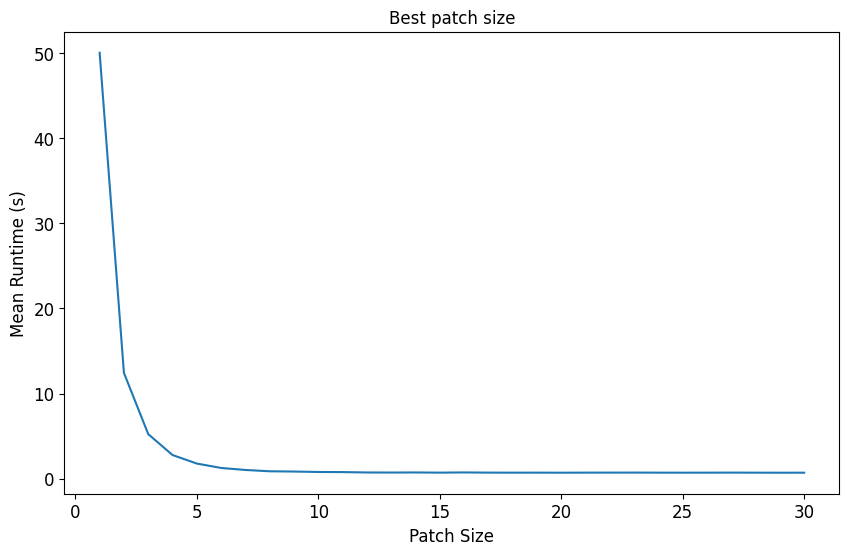
\includegraphics[width=0.7\textwidth]{template-2/best_patch_size.png}
    \caption{Mean Runtime vs. Patch Size - Finding best patch size}
    \label{fig:best_patch_size}
\end{figure}

Based on figure~\ref{fig:best_patch_size}, one can tell that the runtime seems to converge starting from a patch size of 10. The minimum and therefore best patch size according to the numbers provided in table~\ref{tab:best_patch_size}, is 29 which leads to an average runtime of 0.702 seconds. 

\section{Speed-up Analysis}

\subsection{Absolute speed up}

One can calculate the absolute speed up by computing $S_{a}^{A_i}(n, p) = \frac{T_{seq}^*(n)}{T_{par}(n, p)} $. \\

Algorithm sequential:
\begin{align*}
    &T_{\text{seq}}^*(n) = O(n \log n) \\
    &T^*_{\text{seq}}(1000) = O(1000 \log 1000) \approx 6907.76
\end{align*}

Algorithm A1:
\begin{align*}
    &T^{A_1}_{\text{par}}(n, p) = O\left(\frac{n \log n}{p} + \log n\right) \\
    &T^{A_1}_{\text{par}}(1000, 4) \approx 1733.85 \\
    &T^{A_1}_{\text{par}}(1000, 16) \approx 438.64 \\
    &T^{A_1}_{\text{par}}(1000, 64) \approx 114.84
\end{align*}

\begin{align*}
    &S_{a}^{A_1} (1000, 4) = \frac{6907.76}{1733.85} \approx 3.98\\
    &S_{a}^{A_1} (1000, 16) = \frac{6907.76}{438.64} \approx 15.74\\
    &S_{a}^{A_1}(1000, 64) = \frac{6907.76}{114.84} \approx 60.15
\end{align*}

Algorithm A2:
\begin{align*}
    &T^{A_2}_{\text{par}}(n, p) = O\left(\frac{n \log n}{p} + n\right) \\
    &T^{A_2}_{\text{par}}(1000, 4) \approx 2726.94 \\
    &T^{A_2}_{\text{par}}(1000, 16) \approx 1431.73 \\
    &T^{A_2}_{\text{par}}(1000, 64) \approx 1107.93
\end{align*}

\begin{align*}
    &S_{a}^{A_2} (1000, 4) = \frac{6907.76}{2726.94} \approx 2.53\\
    &S_{a}^{A_2} (1000, 16) = \frac{6907.76}{1431.73} \approx 4.82\\
    &S_{a}^{A_2} (1000, 64) = \frac{6907.76}{1107.93} \approx 6.23
\end{align*}

\subsection{Parallel Efficiency}

One can calculate the parallel efficiency by computing $E^{Ai} (n, p) = \frac{S_{a}^{A_i} (n, p)}{p} $. \\

Algorithm A1:
\begin{align*}
    &E^{A_1}(1000, 4) = \frac{S_{a}^{A_1} (1000, 4)}{4} \approx 1.0 \\
    &E^{A_1}(1000, 16) = \frac{S_{a}^{A_1} (1000, 16)}{16} \approx 0.98 \\
    &E^{A_1}(1000, 64) = \frac{S_{a}^{A_1}(1000, 64)}{64} \approx 0.94
\end{align*}

Algorithm A2:
\begin{align*}
    &E^{A_2} (1000, 4) = \frac{S_{a}^{A_2} (1000, 4)}{4} \approx 0.63 \\
    &E^{A_2} (1000, 16) = \frac{S_{a}^{A_2} (1000, 16)}{16} \approx 0.30 \\
    &E^{A_2} (1000, 64) = \frac{S_{a}^{A_2} (1000, 64)}{64} \approx 0.1
\end{align*}



\subsection{Potential Speed-up}

According to Amdahl's Law the potential speed up is bounded by the sequential fraction of the code.\\
\newpage
Algorithm A1:\\
The sequential fraction of A1 is $s_1 = \frac{\log n}{\frac{n \log n}{p} + \log n} = \frac{p}{n+p}$.

\begin{align*}
    &S^{A_1}(n,p) = \frac{1}{s_1 + \frac{1-s_1}{p}} \leq \frac{1}{s_1} = \frac{1}{\frac{p}{n+p} + \frac{1-\frac{p}{n+p}}{p}} \leq \frac{1}{\frac{p}{n+p}}
\end{align*}

Algorithm A2:\\
The sequential fraction of A2 is $s_2 = \frac{\log n}{\frac{n \log n}{p} + n} = \frac{\log n * p}{n*(\log n + p)}$.

\begin{align*}
    &S^{A_2}(n,p) = \frac{1}{s_2 + \frac{1-s_2}{p}} \leq \frac{1}{s_2} = \frac{1}{\frac{\log n * p}{n*(\log n + p)} + \frac{1-\frac{\log n * p}{n*(\log n + p)}}{p}} \leq \frac{1}{\frac{\log n * p}{n*(\log n + p)}}
\end{align*}

However, in the solution above "p" is still involved. Therefore, we decided to use a different approach and take a look at the ratio of the sequential part of the algorithms (in terms of O notation) and take the ratio to the best performing sequential algorithm.\\

Algorithm A1:\\
The sequential part of A1 is $s_1 = \log n$.

\begin{align*}
    &S^{A_1}(n) = \frac{n \log n}{\log n} = n
\end{align*}


Algorithm A2:\\
The sequential fraction of A2 is $s_2 = n$.

\begin{align*}
    &S^{A_2}(n) = \frac{n \log n}{n} = \log n
\end{align*}

\section{Weak Scaling Analysis}

\subsection{Growth of input size}

\begin{align*}
    & O(\frac{n^4}{p}) = O(w)\\ 
    & \frac{n^4}{p} = w \\
    & n^4 = pw \\
    & n = {(pw)}^{\frac{1}{4}}
\end{align*}

Since the average work per processor is w and the parallel algorithm runs in $O(\frac{n^4}{p})$, n needs to increase as the fourth root of the product of w and p to keep the average work at O(n).

\subsection{Input size for different p}

Given that n=100 when p=1, the various input sizes for different numbers of processors can be computed as follows. This time we decided to perform the calculations in R closely following the code presented in the lecture, as can be seen in listing~\ref{lst:r_code}.

\begin{lstlisting}[language=R, caption={Calculation n for various values of p}, label={lst:r_code}]
n <- 100
w <- n^4
df <- data.frame(p=c(2,4,8,16,128))
df$n <- ceiling((df$p*w)^(1/4))
print(df)
\end{lstlisting}

Table~\ref{tab:input_sizes} shows the output of the code and presents the necessary input size for various numbers of cores.

\begin{table}[htbp]
    \centering
    \label{tab:input_sizes}
    \begin{tabular}{cc}
    \toprule
    $p$ & $n$ \\
    \midrule
    2 & 119 \\
    4 & 142 \\
    8 & 169 \\
    16 & 200 \\
    128 & 337 \\
    \bottomrule
    \end{tabular}
    \caption{Required input sizes for different numbers of processors}
\end{table}

\newpage
\section*{Appendix}
\subsection*{System Information}

\begin{lstlisting}[language=,caption={Output of `lscpu` command}]
bopc23s9@hydra-head:~$ lscpu

Architecture:                    x86_64
CPU op-mode(s):                  32-bit, 64-bit
Byte Order:                      Little Endian
Address sizes:                   46 bits physical, 48 bits virtual
CPU(s):                          16
On-line CPU(s) list:             0-15
Thread(s) per core:              1
Core(s) per socket:              16
Socket(s):                       1
NUMA node(s):                    1
Vendor ID:                       GenuineIntel
CPU family:                      6
Model:                           85
Model name:                      Intel(R) Xeon(R) Gold 6130 CPU @ 2.10GHz
Stepping:                        4
CPU MHz:                         1000.151
CPU max MHz:                     3700.0000
CPU min MHz:                     1000.0000
BogoMIPS:                        4200.00
L1d cache:                       512 KiB
L1i cache:                       512 KiB
L2 cache:                        16 MiB
L3 cache:                        22 MiB
NUMA node0 CPU(s):               0-15
\end{lstlisting}

\subsection*{Raw Data}

\begin{table}[h]
\centering
\csvautotabular[separator=semicolon]{output_exp22_1.csv}
\caption{Output 2.2.1}
\label{tab:yourlabel}
\end{table}

\begin{table}[h]
\centering
\csvautotabular[separator=semicolon]{output_exp22_2.csv}
\caption{Output 2.2.2}
\label{tab:yourlabel}
\end{table}

\begin{table}[h]
\centering
\csvautotabular[separator=semicolon]{output_exp23.csv}
\caption{Output 2.3}
\label{tab:yourlabel}
\end{table}

\begin{table}[h]
\centering
\csvautotabular[separator=semicolon]{output_exp24_1.csv}
\caption{Output 2.4 Part 1}
\label{tab:yourlabel}
\end{table}

\begin{table}[h]
\centering
\csvautotabular[separator=semicolon]{output_exp24_2.csv}
\caption{Output 2.4 Part 2}
\label{tab:yourlabel}
\end{table}


\end{document}

